\chapter{Développement du système de traduction automatique}


Après la construction d'\textbf{OpenRuund} présentée au chapitre précédent, cette partie du travail est consacrée au développement du système de traduction automatique. L'objectif est de mettre en œuvre une approche de \ac{TAN} adaptée au contexte des \ac{LFR} en s'appuyant sur des modèles multilingues préentraînés.

Le développement du système comprend l'ensemble des opérations nécessaires à la transformation du corpus en données exploitables pour l'apprentissage automatique, à l'adaptation des modèles retenus, à leur entraînement ainsi qu'à l'évaluation de leurs performances. Une fois le modèle le plus performant identifié, celui-ci est intégré dans une application permettant la traduction automatique.

La Figure~\ref{fig:pipeline_systeme} présente le pipeline global adopté pour le développement du système de traduction automatique.

\begin{figure}[H]
    \centering
    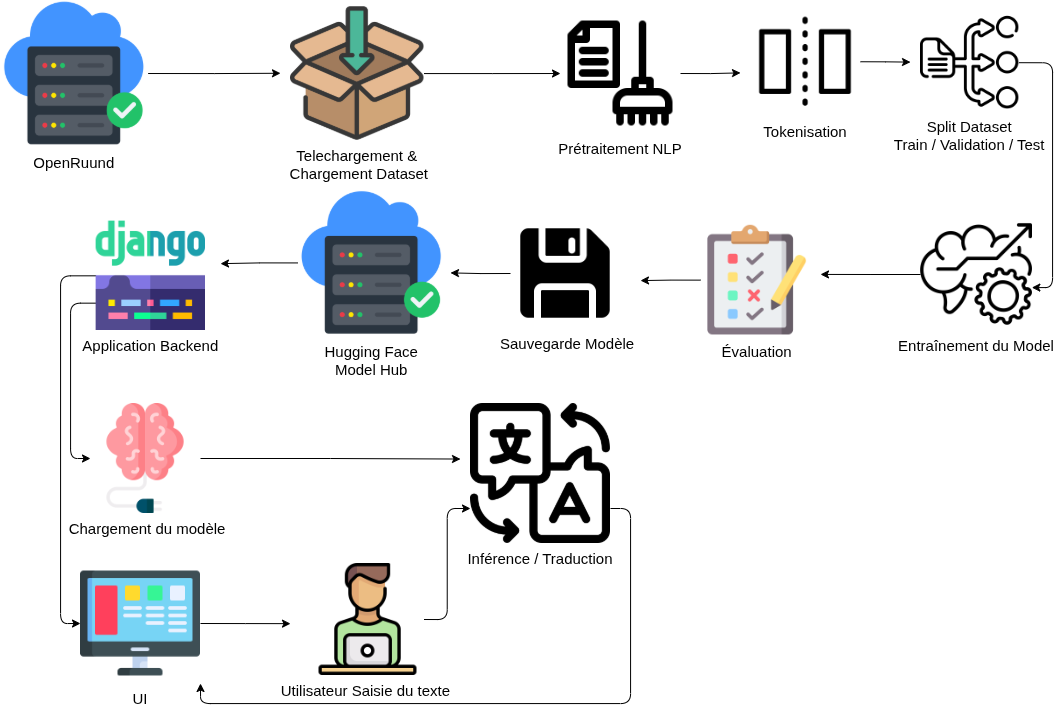
\includegraphics[width=0.70\textwidth]{Images/pipeline_systeme.png}
    \caption[Pipeline global du système de traduction automatique]{Pipeline global du système de traduction automatique}
    \label{fig:pipeline_systeme}
\end{figure}
\section{Préparation des données pour l'entraînement}

Avant l'entraînement des modèles de \ac{TAN}, le corpus OpenRuund a fait l'objet d'une phase de préparation visant à améliorer la qualité des données fournies aux modèles. Cette étape est essentielle dans les systèmes de \ac{TAN}, car la qualité des données d'apprentissage influence directement les performances du modèle. Le processus mis en œuvre comprend la normalisation des textes ainsi que le filtrage des phrases afin de réduire les incohérences présentes dans le corpus.

\subsection{Objectifs du prétraitement}

Le prétraitement constitue une étape fondamentale dans le développement des systèmes de \ac{TAN}. Les modèles de traduction apprennent à partir des relations observées entre les phrases sources et cibles ; par conséquent, la présence de données bruitées ou incohérentes peut dégrader l'apprentissage et affecter la qualité des traductions générées.

Dans le cadre de cette étude, le prétraitement vise principalement à homogénéiser la représentation des textes et à éliminer les éléments susceptibles d'introduire des erreurs lors de l'entraînement. Cette opération permet d'obtenir un corpus plus cohérent, facilitant ainsi l'apprentissage des correspondances linguistiques entre le ruund et le français.

Par ailleurs, la réduction du bruit dans les données contribue à améliorer la qualité générale du corpus. Les doublons, les phrases vides, les séquences anormalement longues ou encore les paires de phrases présentant un déséquilibre important entre les deux langues peuvent introduire des biais dans le processus d'apprentissage. Leur suppression permet de conserver uniquement les exemples les plus pertinents pour l'entraînement des modèles.

\subsection{Normalisation des textes}

Dans un premier temps, une normalisation Unicode de type \ac{NFC}  a été effectuée. Cette opération permet d'uniformiser la représentation interne des caractères Unicode et d'éviter que des caractères visuellement identiques soient encodés de manière différente.

Ensuite, l'ensemble des textes a été converti en minuscules. Cette transformation réduit la variabilité artificielle du vocabulaire en évitant que des mots identiques soient considérés comme différents uniquement en raison de l'utilisation de majuscules.

Une phase de nettoyage des caractères a également été réalisée. Les caractères spéciaux non pertinents ont été supprimés tandis que les principaux signes de ponctuation utiles à la structure des phrases, notamment les points, les virgules, les points d'interrogation, les points d'exclamation et les apostrophes, ont été conservés.

Enfin, les espaces superflus ont été éliminés. Les séquences de plusieurs espaces consécutifs ont été remplacées par un espace unique et les espaces présents en début ou en fin de phrase ont été supprimés. Cette opération permet d'obtenir des textes homogènes et prêts pour les étapes ultérieures d'entraînement.

Le script implémentant ces opérations de normalisation est présenté en annexe (Listing~\ref{code:pretraitement-textes}).

\subsection{Filtrage du corpus}

Après la normalisation des textes, plusieurs opérations de filtrage ont été appliquées afin de conserver uniquement les paires de phrases répondant aux critères de qualité définis pour cette étude.

\subsubsection{Suppression des doublons}

Les paires de phrases identiques apparaissant plusieurs fois dans le corpus ont été supprimées. Cette opération permet d'éviter une surreprésentation de certains exemples durant l'apprentissage et contribue à améliorer la diversité des données utilisées pour l'entraînement.

\subsubsection{Suppression des phrases vides}

Les phrases ne contenant aucun mot après les opérations de prétraitement ont été retirées du corpus. Les paires comportant une phrase vide dans l'une des deux langues ne fournissent aucune information utile au modèle et peuvent perturber le processus d'apprentissage.

\subsubsection{Filtrage par longueur des phrases}

Un seuil maximal de 80~mots a été fixé pour chacune des langues. Les paires dont la phrase ruund ou la phrase française dépassait cette limite ont été supprimées. Cette contrainte permet d'écarter les séquences exceptionnellement longues susceptibles d'augmenter la complexité de l'entraînement et de générer des déséquilibres dans les données.

\subsubsection{Filtrage par ratio de longueur}

Un contrôle du rapport de longueur entre les phrases alignées a également été réalisé. Pour chaque paire de phrases, le ratio entre la longueur de la phrase source et celle de la phrase cible a été calculé :
\begin{equation*}
\frac{\max(L_{\text{ruund}},\,L_{\text{français}})}{\min(L_{\text{ruund}},\,L_{\text{français}})} \leq 2
\end{equation*}

Les paires présentant un ratio supérieur à~2 dans l'un ou l'autre sens ont été éliminées.

Cette opération permet de détecter les alignements potentiellement incorrects ou les traductions incomplètes. En effet, des différences excessives de longueur entre deux phrases supposées équivalentes peuvent indiquer une mauvaise correspondance entre les segments alignés. Le maintien d'un ratio inférieur ou égal à~2 contribue ainsi à préserver la cohérence linguistique du corpus parallèle utilisé pour l'entraînement des modèles.

L'ensemble des opérations de filtrage décrites ci-dessus est implémenté dans le script présenté en annexe (Listing~\ref{code:filtrage-phrases}).